\documentclass{ctexart}
\usepackage{geometry}
\usepackage{amsmath}
\usepackage{listings}
\usepackage[dvipsnames]{xcolor}
\usepackage{cite}
\usepackage{diagbox}
\usepackage{fancyhdr} % 加载fancyhdr宏包,用于设置页眉和页脚
\pagestyle{fancy} % 设置页面样式
\fancyhf{} % 清除默认的页眉和页脚的内容
\fancyfoot[C]{\thepage} 
\renewcommand{\headrulewidth}{0pt} % 将页眉的横线宽度设置为0pt
\usepackage[left=2.5cm,right=2.5cm,top=2.5cm,bottom=2.5cm]{geometry}
\usepackage{graphicx}
\usepackage{longtable}
\usepackage{tabularx}
\usepackage{float}
\usepackage{amsmath}%引用宏包要放在documentclass后面,否则报错
\usepackage{hyperref}
\usepackage{bm}
\usepackage{amssymb}
\usepackage{esint}
\usepackage{booktabs}
%\usepackage{subfiles}%用于分章节管理引用,使各章节引用来源于各自的文件,编号相互独立
\usepackage{amsthm}
\title{数字电路实验\quad 实验二报告}
\author{Leo}
\date{\today}

\begin{document}
\maketitle
\section{实验内容}
用逻辑门实现设计2421BCD码的检测电路:
\begin{enumerate}
    \item 列出2421BCD码的真值表
    \item 给出电路实现方案
    \item 调试电路,实现当检测到有效码时,LED灯不亮;当检测到无效码时,LED灯亮起
\end{enumerate}
\section{实验器材}
Pocketlab、电脑、导线若干、剥线钳、镊子、限流电阻一个、红色LED灯一个、7404芯片一个、7400芯片一个、7420芯片一个。芯片的引脚图如下所示
\begin{figure}[H]
    \centering
    \begin{minipage}{0.25\textwidth}
    \centering
           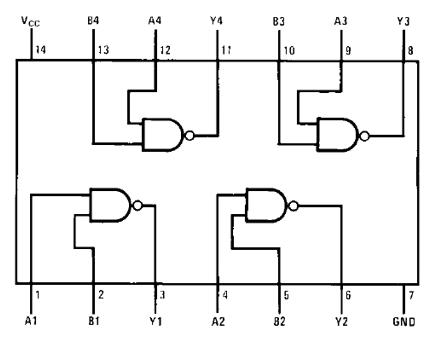
\includegraphics[width=0.8\textwidth]{fig/7400.png}
           \caption{7400}
    \label{}
    \end{minipage}
    \hspace{0.05\textwidth}
    \begin{minipage}{0.25\textwidth}
    \centering
           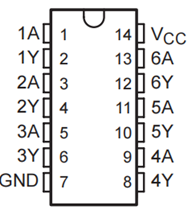
\includegraphics[width=0.8\textwidth]{fig/7404.png}
           \caption{7404}
    \label{}
    \end{minipage}
     \hspace{0.05\textwidth}
    \begin{minipage}{0.28\textwidth}
    \centering
           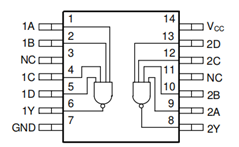
\includegraphics[width=0.8\textwidth]{fig/7420.png}
           \caption{7420}
    \label{}
    \end{minipage}
\end{figure}
\section{实验原理}
题目要求识别2421BCD码中的伪码,若设输入变量为A,B,C,D,输出为F,并规定伪码输出为1,有效码输出为0,则可以列出如下真值表

\begin{longtable}{|p{2cm}<{\centering}| p{2cm}<{\centering} |p{2cm}<{\centering}| p{2cm}<{\centering} |p{2cm}<{\centering}|}%手动调间距
\caption{真值表}
\hline
  A & B & C & D & F \\
\hline
  0 & 0 & 0 & 0 & 0 \\
\hline
  0 & 0 & 0 & 1 & 0 \\
\hline
  0 & 0 & 1 & 0 & 0 \\
\hline
  0 & 0 & 1 & 1 & 0 \\
\hline
  0 & 1 & 0 & 0 & 0 \\
\hline
  1 & 0 & 1 & 1 & 0 \\
\hline
  1 & 1 & 0 & 0 & 0 \\
\hline
  1 & 1 & 0 & 1 & 0 \\
\hline
  1 & 1 & 1 & 0 & 0 \\
\hline
  1 & 1 & 1 & 1 & 0 \\
\hline
  0 & 1 & 0 & 1 & 1 \\
\hline
  0 & 1 & 1 & 0 & 1 \\
\hline
  0 & 1 & 1 & 1 & 1 \\
\hline
  1 & 0 & 0 & 0 & 1 \\
\hline
  1 & 0 & 0 & 1 & 1 \\
\hline
  1 & 0 & 1 & 0 & 1 \\
\hline
\end{longtable}
对应真值表可以做出卡诺图
\begin{table}[H]
    \centering
    \caption{卡诺图}
    \begin{tabular}{|c|c|c|c|c|}
\hline
\diagbox{AB}{CD} & 00 & 01 & 11 & 10 \\
\hline
00 & 0 & 0 & 0 & 0  \\
\hline
01 & 0 & 1 & 1 & 1  \\
\hline
11 & 0 & 0 & 0 & 0  \\
\hline
10 & 1 & 1 & 0 & 1  \\
\hline
\end{tabular}
    \label{tab:卡诺图}
\end{table}
写出逻辑函数的表达式
\begin{equation}
    \begin{aligned}
F &=\sum m(5,6,7,8,9,10)\\
&=AB'C'+AB'D'+A'BD+A'BC\\
&=AB'(C'+D')+A'B(C+D)\\   
&=AB'(CD)'+A'B(C'D')'
    \end{aligned}
\end{equation}
最后一行不是最简表达式,但是这样写可以尽可能多地使用与非门,节省不同种芯片的使用量。从表达式中可以看出,主要用到了非门和与非门,有一个或门,也可以用与非来代替。于是我们选用7400(2输入4与非门)、7404(6非门)和7420(4输入2与非门)。
\section{电路设计与实现}
\subsection{电路仿真图}
在Multisim中连接好电路仿真图
\begin{figure}[H]
    \centering
    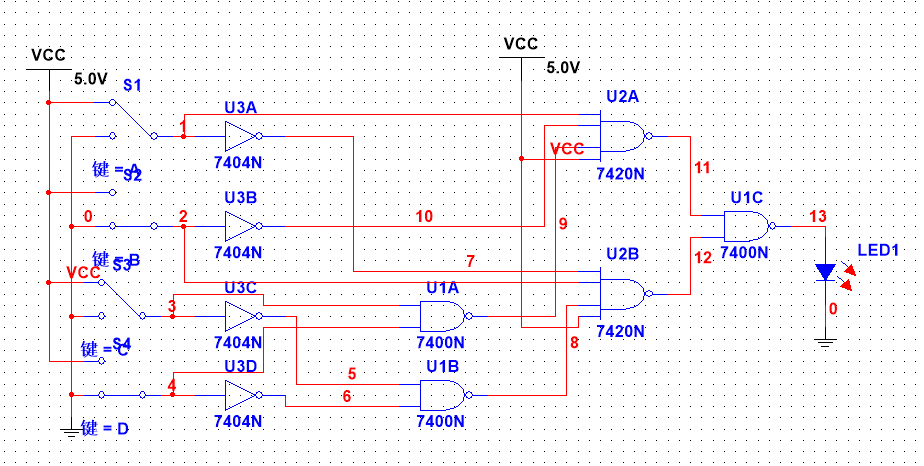
\includegraphics[width=0.75\linewidth]{fig/电路仿真图1.png}
    \caption{电路仿真图1}
    \label{电路仿真图1}
\end{figure}
这里采用键控的方式,实现ABCD四个输入的变换。注意在四输入与非门处,由于实际输入的变量只有三个,所以剩下的一个输入端要接高电平,不影响门的输出。在Multisim中测试,显示设计结果正确。
\subsection{电路实物图}
按电路仿真图搭好实物电路图
\begin{figure}[H]
    \centering
    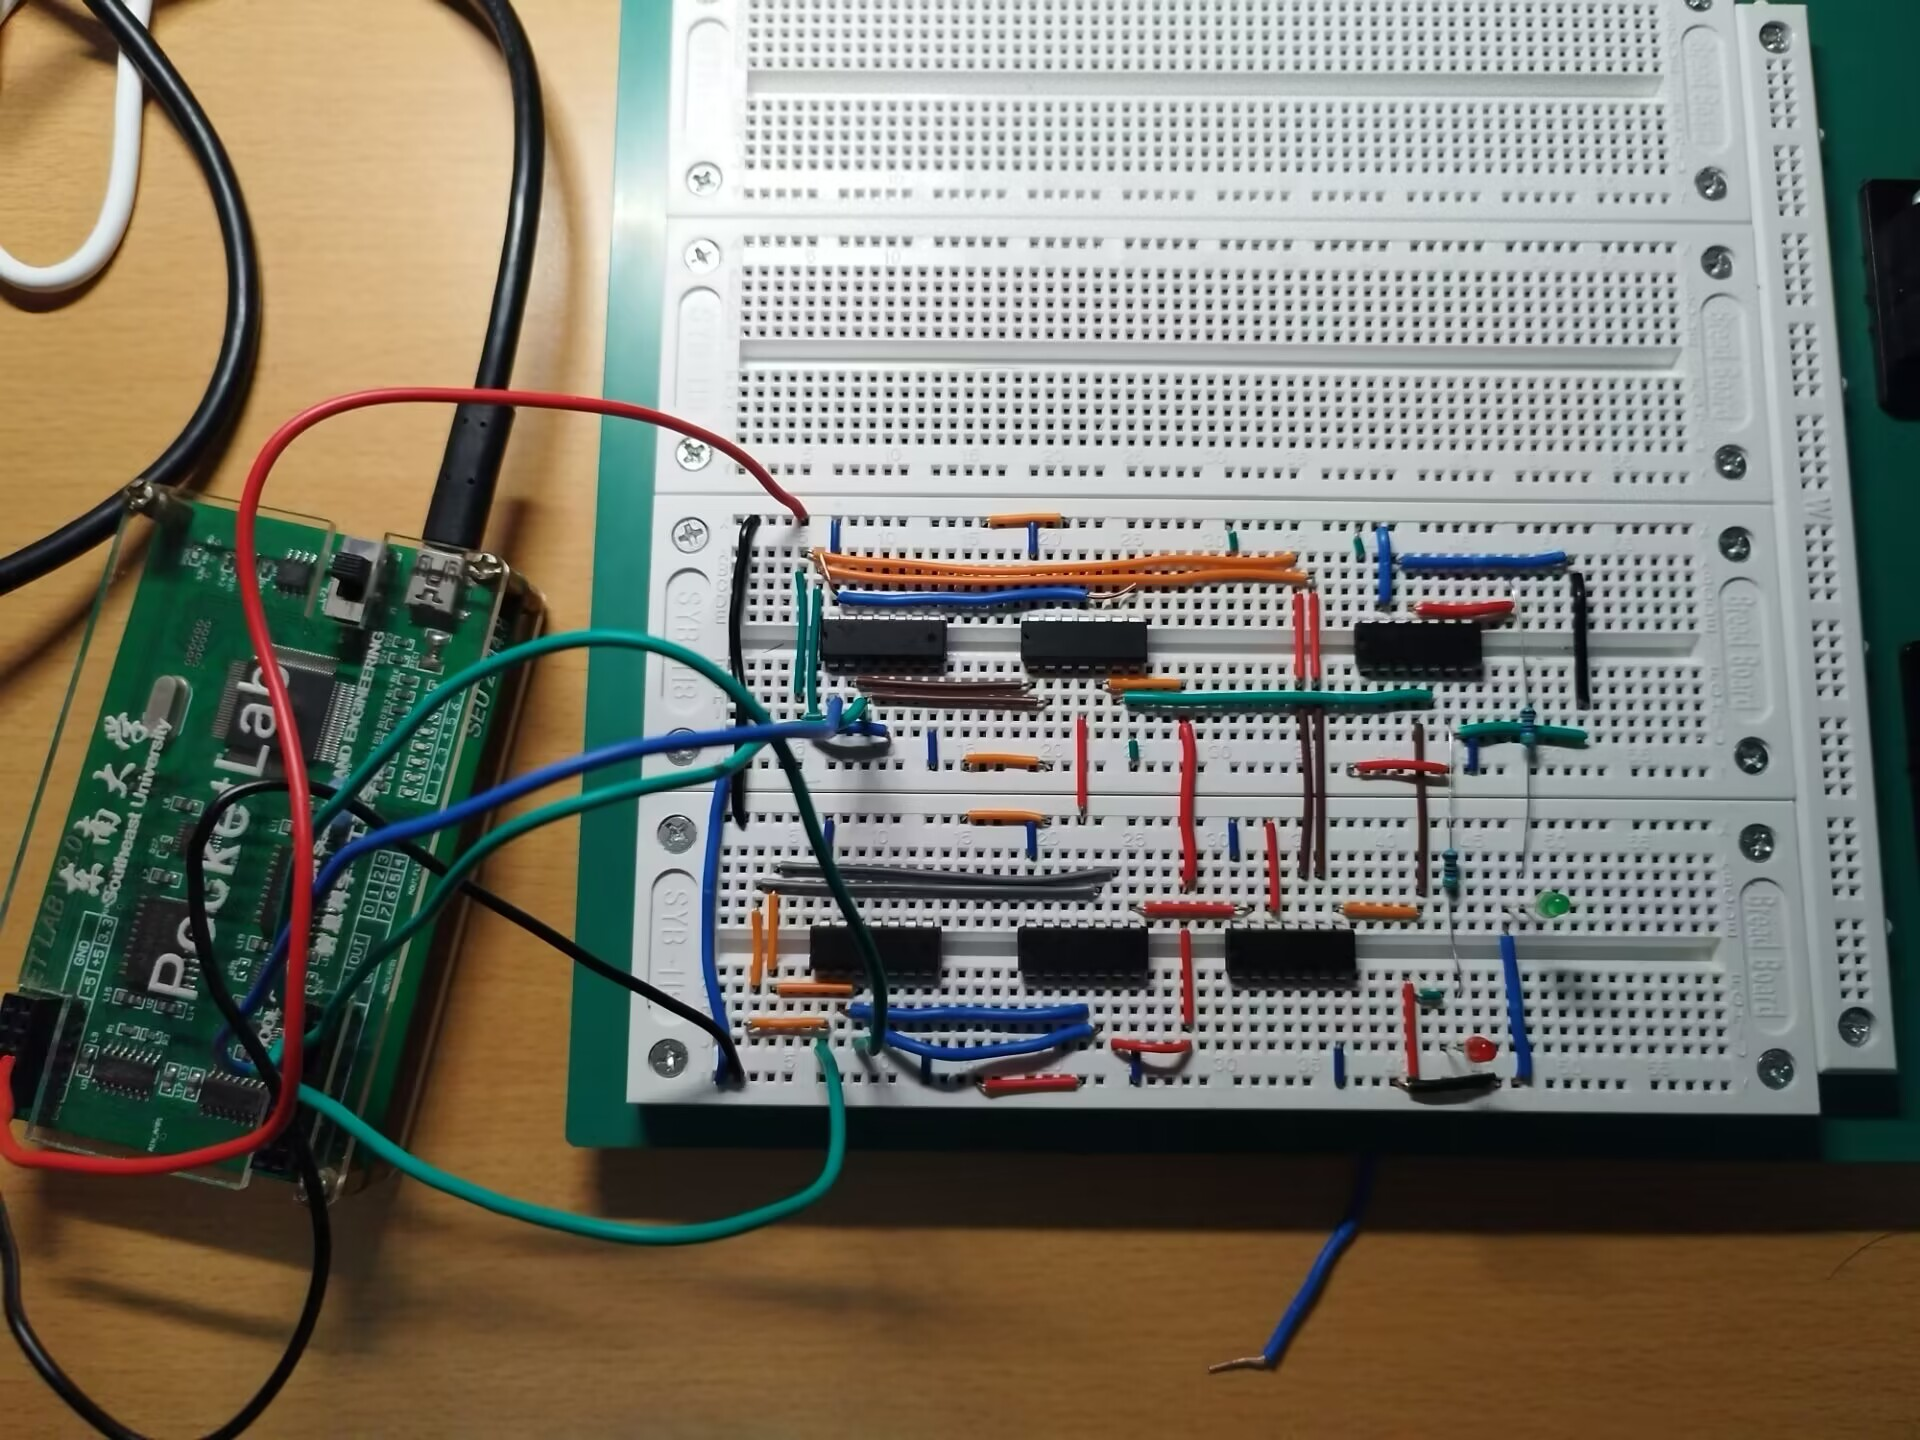
\includegraphics[width=0.75\linewidth]{fig/实物电路图5.jpg}
    \caption{实物电路引脚图}
    \label{实物电路引脚图}
\end{figure}
\section{功能测试}
对搭建好的实物电路进行测试,第一次测试时发现LED灯不亮,经检查是由于看错pocketlab输入高电平的引脚孔,将高电平线引到了GND区。

第二次测试发现,当输入为1000,1001,1010时,输出不对,对比真值表发现,即当AB输入为10时,输出全为0。推测是由于7420芯片的1A端和1B端接法错误导致的。1A端应该始终接在逻辑高电平上,第一版设计是将其接在同一芯片的VCC端;尝试将1A端单独拉出接在高电平上。1B端第一版接法中有较长的引脚暴露且本身引脚较短,可能会接触不良;尝试换一根长线重新连接。

经过上述调整,所有逻辑输入都能产生正确的输出信号。如图是Pocketlab逻辑分析仪的部分实验截图
\begin{figure}[H]
    \centering
    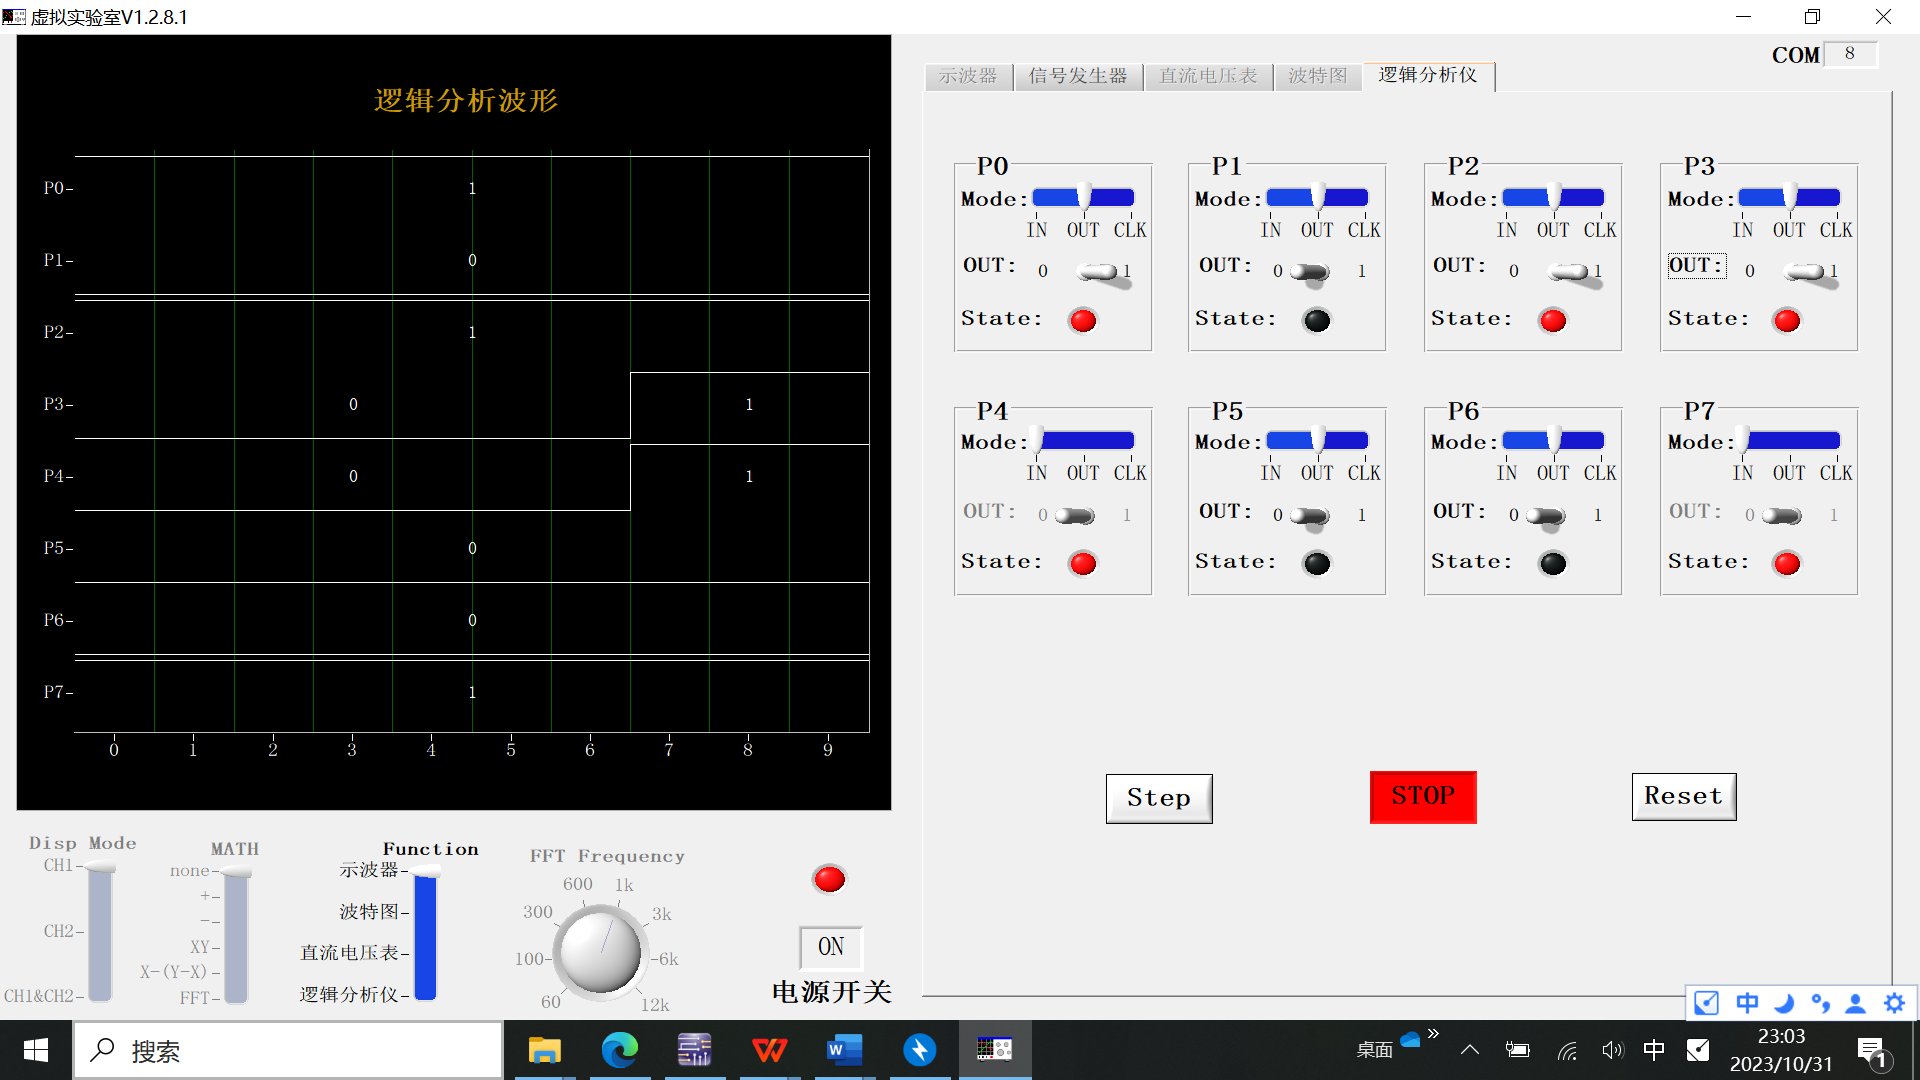
\includegraphics[width=0.75\textwidth]{fig/Pocketlab界面截图1.png}
    \caption{Pocketlab界面截图1}
    \label{Pocketlab界面截图1}
\end{figure}
\begin{figure}[H]
    \centering
    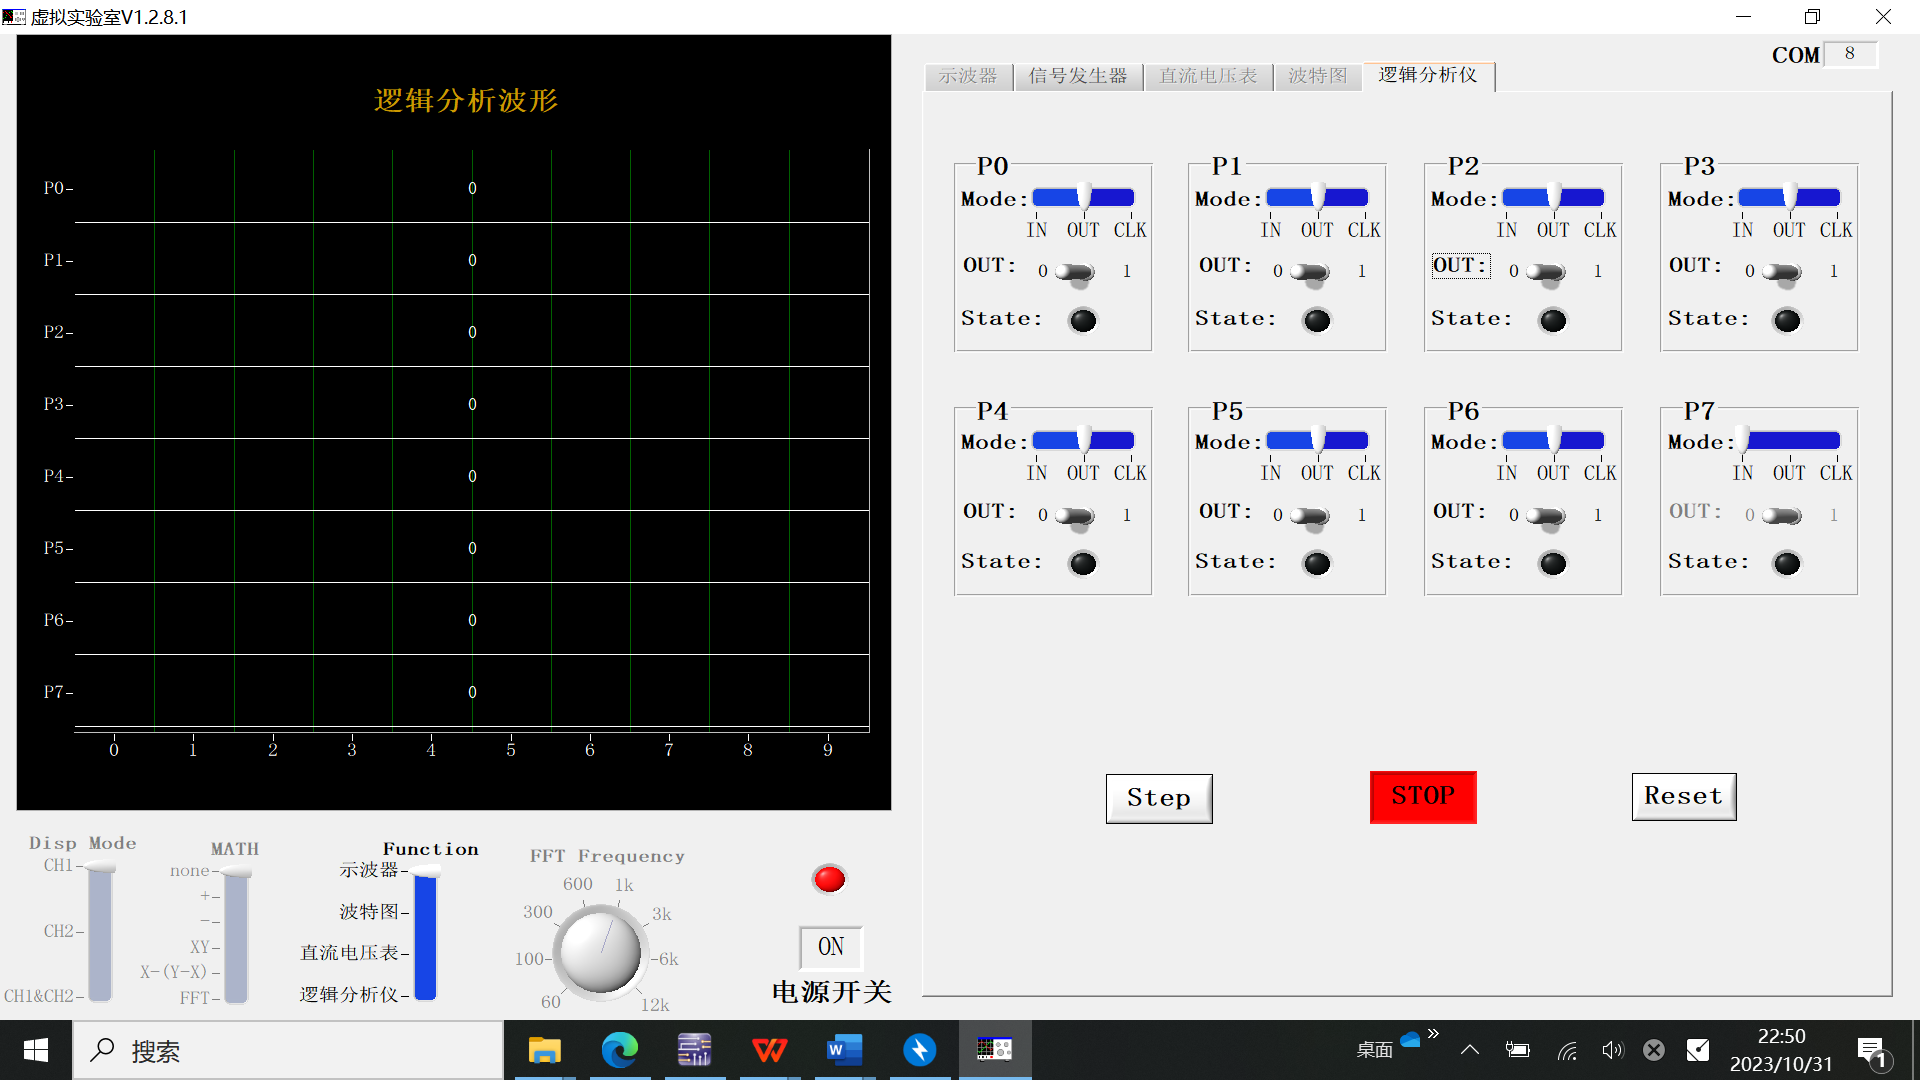
\includegraphics[width=0.75\textwidth]{fig/Pocketlab界面截图2.png}
    \caption{Pocketlab界面截图2}
    \label{Pocketlab界面截图2}
\end{figure}
下面是实物电路图检验2421BCD码的图示
\begin{figure}[H]
    \centering
    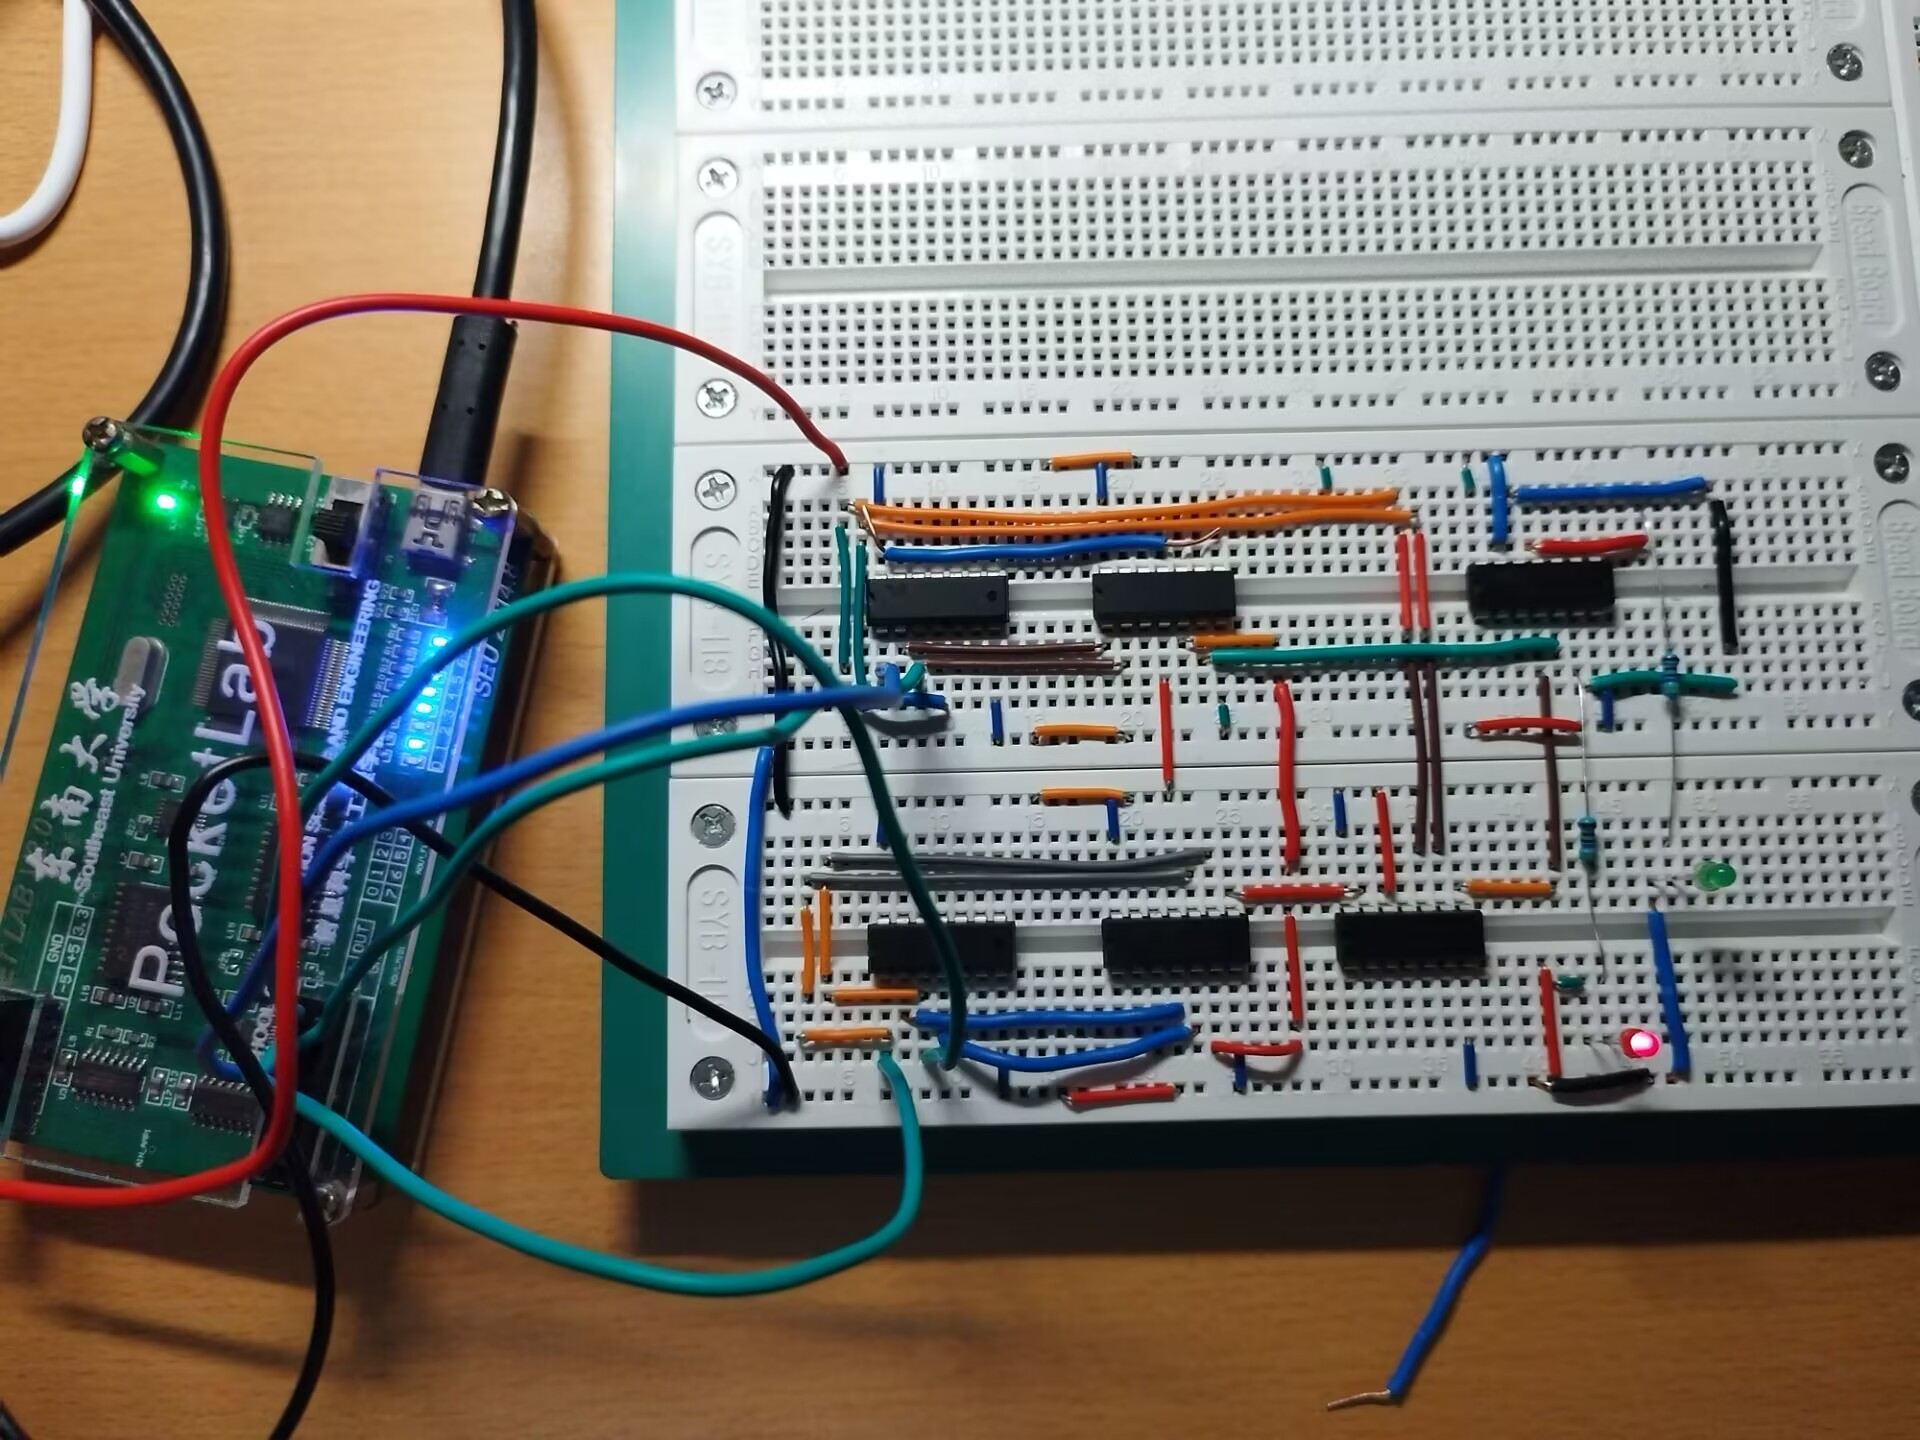
\includegraphics[width=0.6\linewidth]{fig/实物电路图3.jpg}
    \caption{检测到非法码}
    \label{检测到非法码}
\end{figure}
\begin{figure}[H]
    \centering
    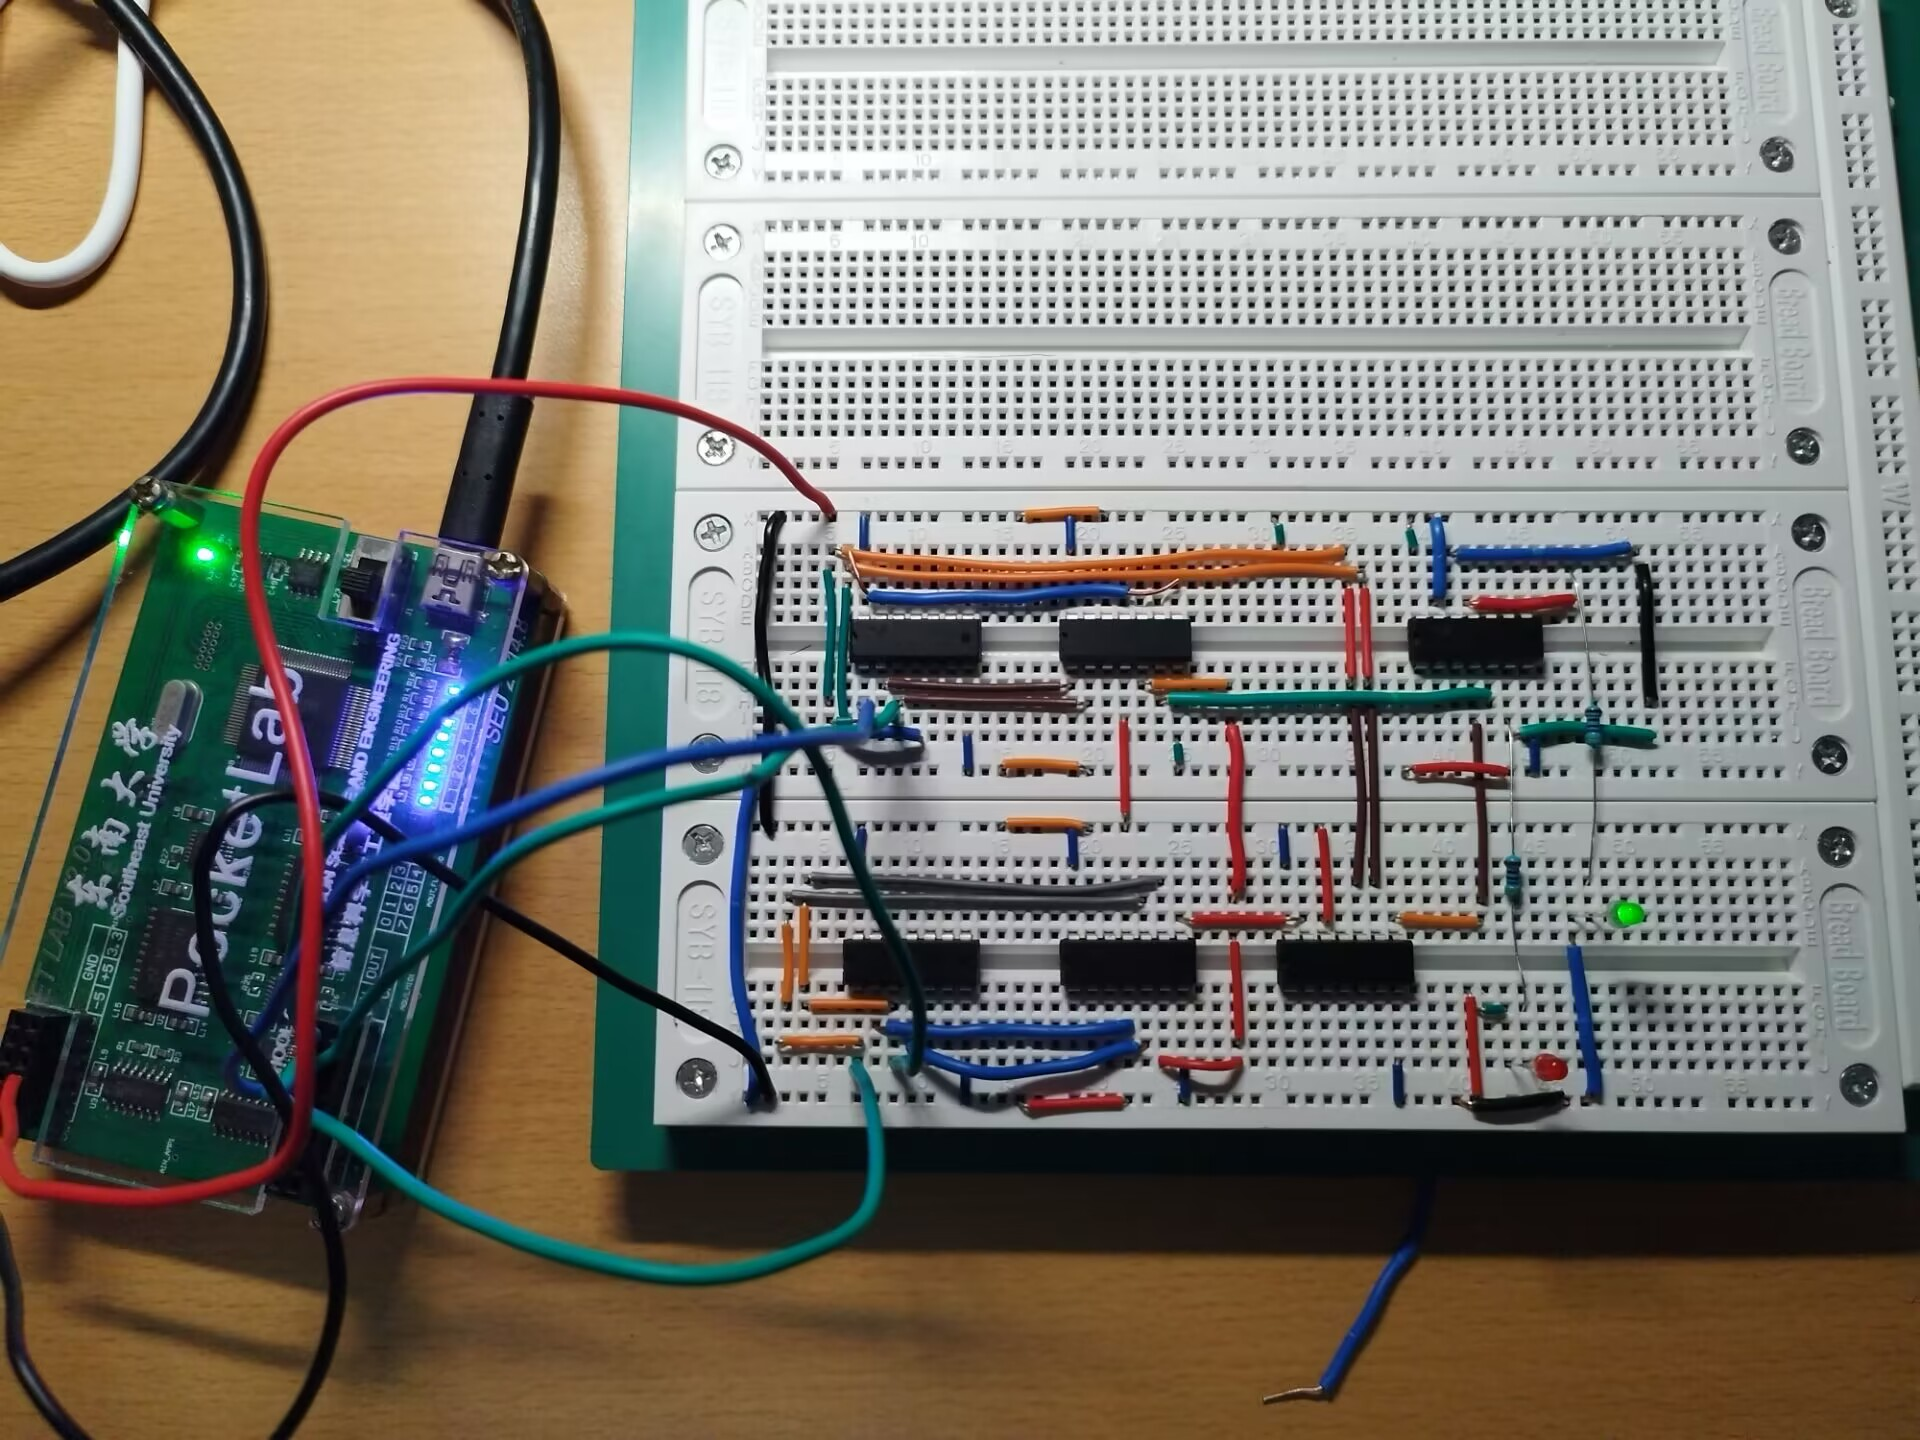
\includegraphics[width=0.6\linewidth]{fig/实物电路图4.jpg}
    \caption{检测到合法码}
    \label{检测到合法码}
\end{figure}
\section{实验总结与反思}
本次实验总体来说较为顺利,需求分析、逻辑表达、电路设计、仿真测试各个环节都没有遇到太大问题。但仍在以下几个方面有待提升
\begin{enumerate}
    \item 走线规范性有待提升。出现了飞线和跳线,线与线之间的交叉也比较频繁;没有让线贴近面包板,看起来比较混乱。这一问题在笔者搭建的第二版电路中尤为严重,而且影响了后续的测试与错误排查,因此笔者选择重新布线,搭建了如图\ref{实物电路引脚图}的电路。
    \item 对实验中遇到的反常之处没有从原理上完全弄懂,仅凭经验猜测可能出现的问题。这样的判断方式在以后处理较大规模电路时可能效率低下。
    \item 出现了高电平线从pockelab地线区引出的低级错误。
\end{enumerate}
补充思考:
1.笔者发现不同电路方案选择的芯片数量不同,对布线会造成很大影响。一般说来,芯片用的多,可以只取芯片的一侧引脚来使用,走线就可以减少;芯片用得少,为了充分利用芯片两侧的所有引脚,就不得不增加导线的数量。

2.本实验要求用门电路实现2421码的检查,输出函数可以写成最小项的或,因此可以用最小项发生器来实现。比如74151数据选择器。通过对数据降维,可以用一片74151以及一个非门实现同样的功能,用线也更加节省。笔者实现了上述电路,并测试成功。如图是仿真电路图和实物电路图
\begin{figure}[H]
    \centering
    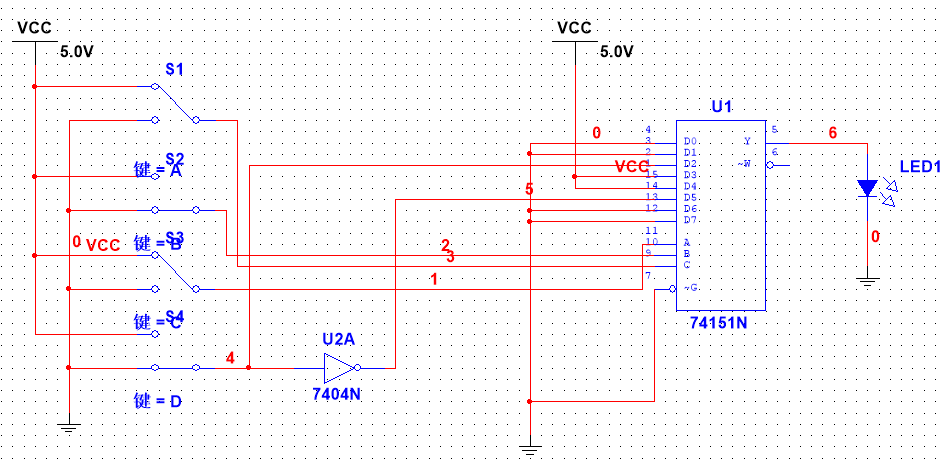
\includegraphics[width=0.6\linewidth]{fig/电路仿真图2.png}
    \caption{电路仿真图2}
    \label{电路仿真图2}
\end{figure}
\begin{figure}[H]
    \centering
    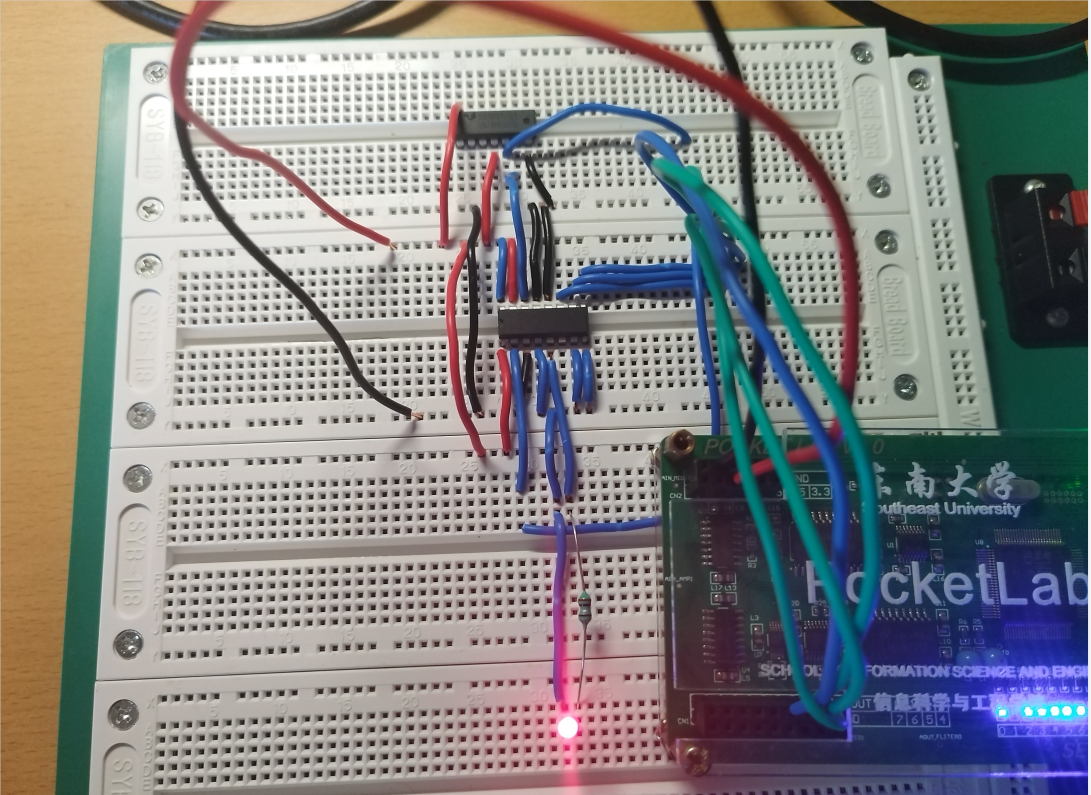
\includegraphics[width=0.6\linewidth]{fig/实物电路图2.png}
    \caption{用74151实现非法码的检验}
    \label{实物电路图2}
\end{figure}
\end{document}